\chapter{Related Philosophy}\label{appendix:philosophy}

\section{The Objective Modelling Assumption}

\begin{figure}[bth]
  \center
  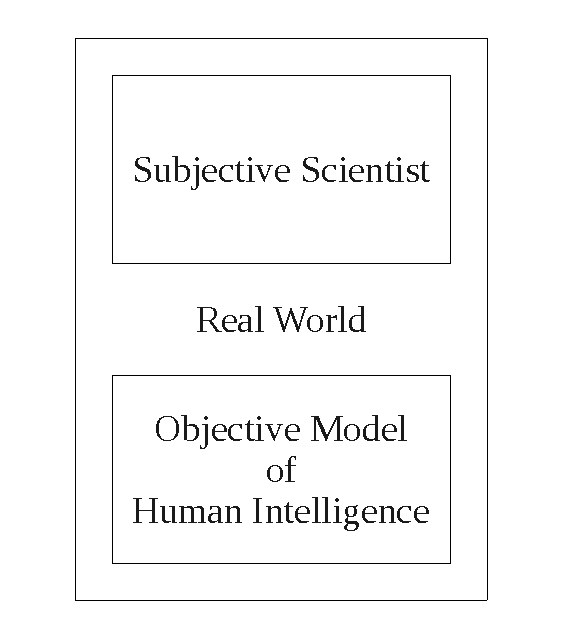
\includegraphics[width=4cm]{gfx/objective_description}
  \caption[The objective-subjective modelling assumption]{The objective-subjective modelling assumption.}
  \label{fig:objective_description}
\end{figure}

We assume that the phenomenon that we are trying to model, namely
human intelligence, is an objective process that we can describe.
This is the objective-subjective philosophical assumption that is
inherent in any objective scientific hypothesis.  We make this
assumption in order to avoid logical problems of circular causality
that occur when trying to find a non-objective description of
reflective thinking.  Figure~\ref{fig:objective_description} shows
how, given the objective assumption, the subjective scientist is part
of the real world, while she is studying an objective phenomenon.
Given the objective-subjective assumption, it would be a grave mistake
to confuse an objective model for reality itself.

\section{Being, Time, and the Verb-Gerund Relationship}

\section{The intensional stance}

\section{Reflective Representations}

\citep{perner:1991}

